\chapter{ReceiptBudget: A System for Managing Personal Finances Based on Receipts}
\label{chap:application}

% ii ok o introducere asa personala?
The idea for ReceiptBudget came out of a necessity most students face when they come to college and have to manage their own money for the first time. They are most often overspending and not keeping good track of their finances. Most existing tools are difficult to use or require a lot of time. Some try to use Excel spreadsheets to record their expenses, but that is tedious and easy to forget to do. Others, like Mint \cite{mint}, that offered very detailed reports and forecasts, would get the information by linking to a bank account. GnuCash \cite{gnucash}, had an extremely complicated system for doing double bookkeeping. Programs like Toshl \cite{toshl} or ExpenseIQ \cite{expenseiq} weren't doing much more than an Excel spreadsheet with a couple of charts, and entering data is not any easier. 

ReceiptBudget is a solution to all these problems and to help people manage their budgets, presented in this thesis. It is  really easy to add expenses by taking a photo of a receipt and having the OCR engine extract the details from the photo. There would have to be lots of reports, which can be filtered by months, shops or items, so that the users could observe spending patterns and hopefully do something about them.

\section{The OCR Engine. Our proposal}
The OCR engine does three things: it preprocesses and normalizes an image containing a receipt, it recognizes the text that is written on each line and then it extracts useful information from that text. 

\subsection{Model design}

\subsubsection{The Random Forest Model}
The random forest was used as a model for the character segmentation problem. The criterion for choosing the best feature to split a node is the information gain (entropy). Trees are grown to their full depth, no pruning or limitation is applied to the branches. 

The other parameters of the random forest were chosen by cross-validation: the number of trees and the number of features to consider when randomly sampling from the feature space. 

\subsubsection{The Support Vector Machine Model}
The SVM was used as a baseline for the character recognition problem. The performance of both linear and radial basis function kernels was evaluated. 

The regularization parameter of the SVM was determined using cross-validation. 

\subsubsection{The Neural Network Model}
Neural networks were used for recognizing the characters. Various models were tried, including Autoencoders, Rectified Linear Units and Dropout. 


\subsection{Document Layout Analysis}
Before any characters can be recognized in a receipt, the image must first be preprocessed and normalized. This is done in several steps. 

The preprocessing consists of binarizing the images, using Otsu's method\cite{otsu1975threshold}, which adapts the threshold based on the histogram of the image. This step is done to remove any noise and speckles from the image. 

The first step in normalization is to straighten the images. The receipts are assumed to be photographed with a mobile phone camera. Users will most often take photos that are slightly rotated. The orientation of the images is assumed to be vertical, so the software will not try to identify if the receipt is horizontal. To straighten the images, they are rotated from -10 to 10 degrees, with a 0.3 angle step, and a horizontal projection (summing the pixel values row-wise) is done for each resulting image. The straight image is assumed to be the one were are the most variations between the peaks and valleys of the histogram, because in the straight image there would be high peaks because of the lines and low valleys because of the space between lines. 

The following step is removing the edges of the image, to keep only the receipt, removing any background. Due to variations in illumination, we cannot simply look for white patches to identify the receipt, because mobile cameras often use flash which gives receipts a blue tint while photos taken indoor close to a source of light have a yellow hue. The approach that was used was to look at the horizontal and vertical projections and to remove the section from the top and bottom that is over a threshold. 

The last step is detecting the lines in the receipt. Because the images are already straight and without edges, all we have to do is identify the peaks in the horizontal histogram in the image.  

The end result of the Document Layout Analysis is shown in figure \ref{fig:receipts}, where we can see a receipt that is given as an input to the engine and the output of the Document Layout Analysis, the normalized image, with the detected lines highlighted.


\begin{figure}
\centering
\begin{subfigure}{0.45\linewidth}
  \centering
  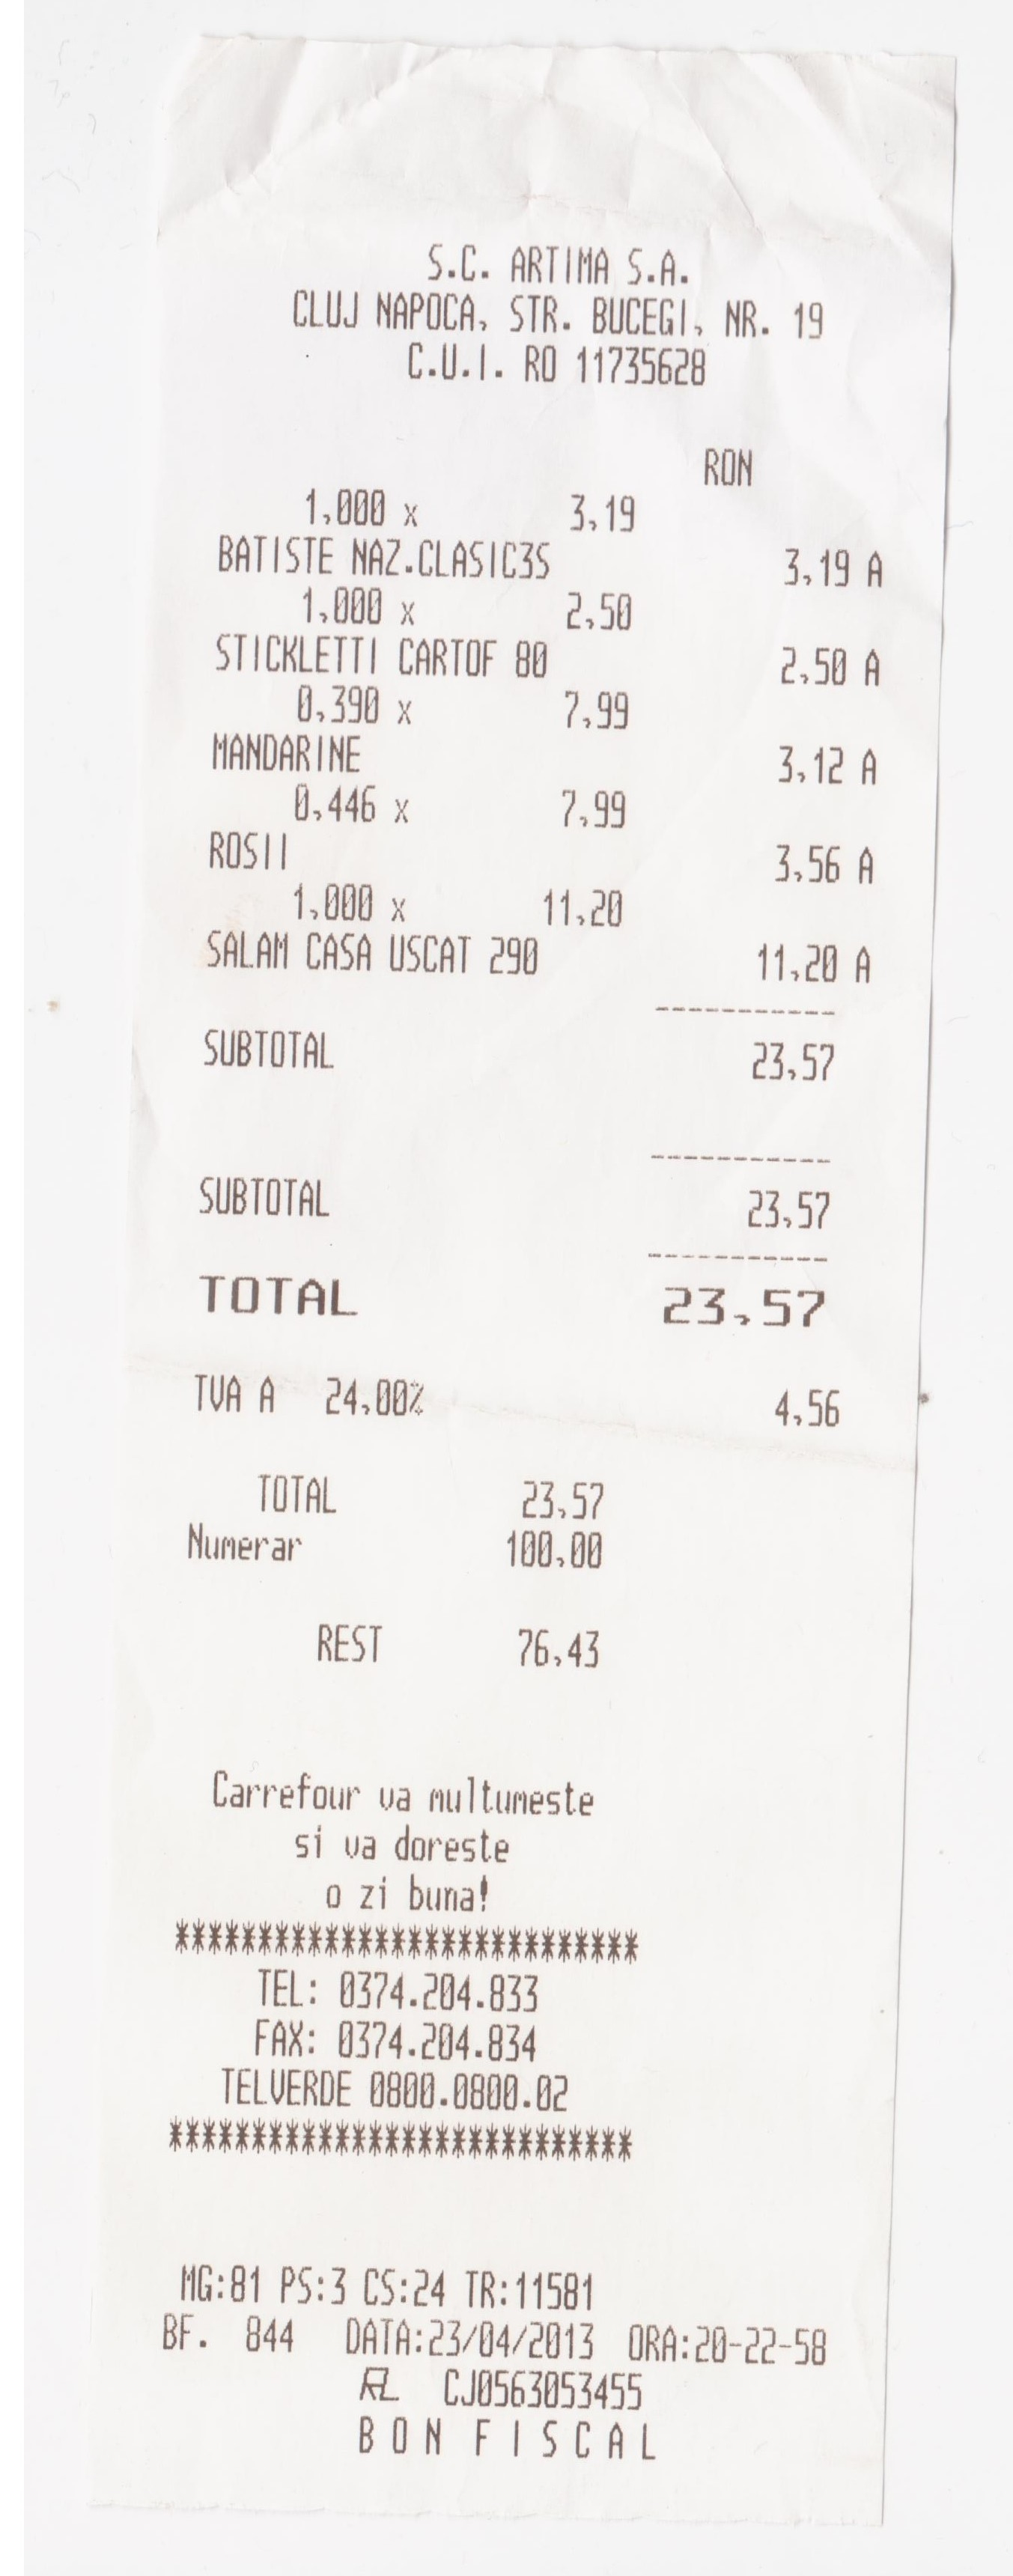
\includegraphics[width=.6\linewidth]{img/bon1.jpg}
  \caption{Example receipt}
  \label{fig:sub1}
\end{subfigure}%
\begin{subfigure}{0.45\linewidth}
  \centering
  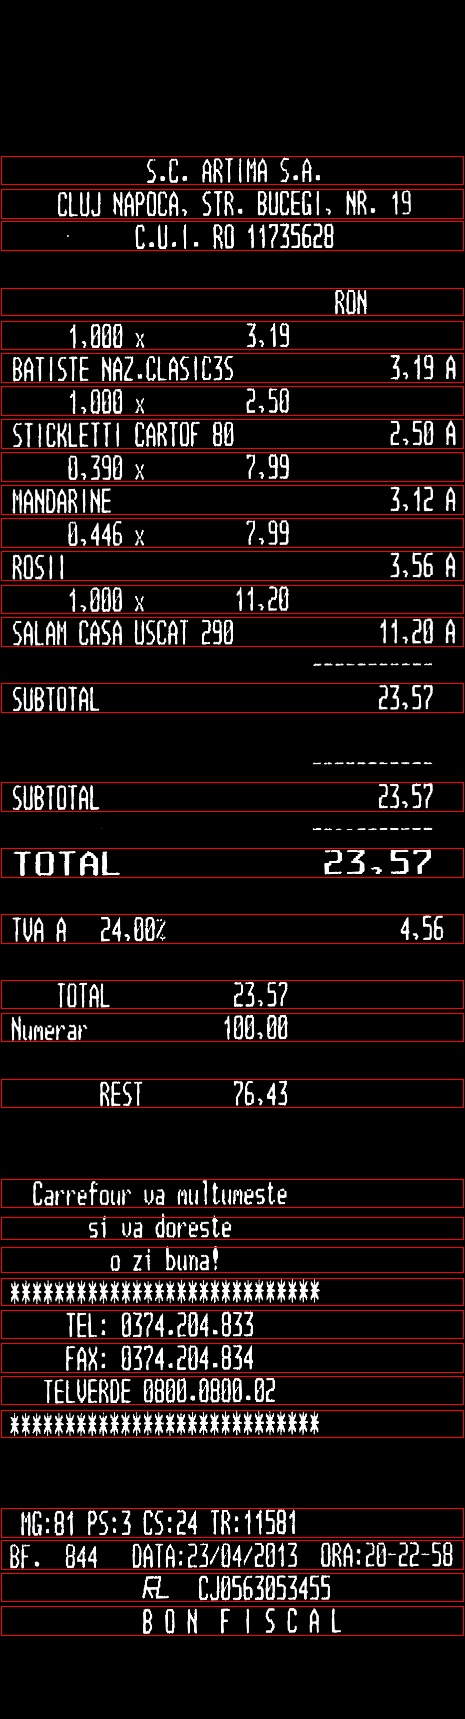
\includegraphics[width=.4\linewidth]{img/cleaned1.jpg}
  \caption{Receipt after passing through normalization}
  \label{fig:sub2}
\end{subfigure}
\caption{\label{fig:receipts}
Figure \ref{fig:sub2} is obtained after edge removal, straightening and binarization of figure \ref{fig:sub1}. Detected lines are shown with red bounding boxes.}
\label{fig:test}
\end{figure}

\subsection{Extracting data from text}
After the text is recognized in images, it must be processed and brought to a usable form. There are 6 relevant pieces of information that can be extracted from a receipt: the name of the shop which emitted the receipt, the address of that shop, the Unique Identifying Code (CUI) given to the company by the government, the items that were bought, the date the sale was made, and the total sum of money paid. 

The approach used in this thesis to extract this information is a simple rule based based system, that looks at each line and checks if it matches some conditions, such as if it matches a regular expression, or the if the count of digits, letters and other characters on the line is in certain ranges, to try to classify each line in one of those categories. 

The name of the shop is identified by searching the line for the following regular expression: 

\begin{lstlisting}
'S\.?C\.?(.+?)(S.?R.?L.?)|(S[:.,]?A[:.,]?)'
\end{lstlisting}

This expression search for anything that starts with \textbf{S.C.} and ends with either a \textbf{S.R.L} or \textbf{S.A.}. Because the dots are small and they are likely to be misclassified or not recognized, they are made optional in the regular expression. Another condition that a line must satisfy is to be in the first 5 lines of the receipt. This is done to prevent detecting any oddly named items that might match this pattern. The only problem with this regular expression is that some shops belong to a different class of entities, such as Kaufland, which is a ``Societate în comandită''.

The unique identifier of the shop can come in multiple forms: it always contains at least 4 digits, sometimes is prefixed by \textbf{C.U.I}, \textbf{C.F.} or \textbf{C.I.F.}, and it must be in the first 6 lines of the receipt. Also, any line containing 8 consecutive digits is considered to be the unique identifier. The regular expression for this is given by:

\begin{lstlisting}
'(C[^\w]?U[^\w]?I[^\w]?)|(C[^\w]?F[^\w]?)|
 (C[^\w]?I[^\w]?F[^\w]?)|
 (COD FISCAL).+? (\d){4,}'
\end{lstlisting}

The address is locating by looking for one of two patterns. If the line is among the first 3 lines in the receipt and it contains the letters \textbf{NR} followed by digits, it is assumed to be an address. To other condition is if it is in the first 7 lines and it starts with either \textbf{STR}, \textbf{CALEA} or \textbf{B-DUL}. These regular expressions are the following:

\begin{lstlisting}
'(STR)|(CALEA)|(B-DUL).(.+?)'
'(NR).(\d+)'
\end{lstlisting}

If the substring \textbf{TVA} is found, the line is marked as a line containing the value added tax. This is not used anywhere else, but it helps reduce false classifications, because the item class is usually similar in structure. 

Totals are identified very simply, by looking for the substring \textbf{TOTAL} or \textbf{SUBTOTAL}.

Dates are identified by looking for a pattern that consists of two to four digits repeated three times, with either periods, commas or slashes between them. Optionally, it can be prefixed with \textbf{DATA}.

\begin{lstlisting}
'DATA?.+?\d{2,4}[.\\-]\d{2,4}[.\\-]\d{2,4}'
'\d{2}[./\\-]\d{2}[./\\-]\d{2,4}'
\end{lstlisting}

Items must occur before the line containing the \textbf{TOTAL}. Items sometimes have the name of the item and its price on the same line, but sometimes they are on two lines. The price part must have at least one character (usually for the currency), the ratio of digits to letters must be greater than one, it must be at least the third line in the receipt, but not in the last seven lines and the line most not contain \textbf{TEL} or \textbf{FAX}. The part with the item name must be at least the fourth line in a receipt, but before the last eight lines, it must have at least five letters and punctuation characters, and it must not contain any of the following \textbf{TEL}, \textbf{FAX}, \textbf{SUBTOTAL}, \textbf{NUMERAR}, \textbf{BRUT}, \textbf{NET} or any of the day names. 

Any other lines are classified as unknown and are not taken into consideration in the subsequent steps.   

\subsection{Data Set and Processing}
The data set was obtained from 20 receipts that were manually annotated with the position of each character in them. In total there are 7045 characters. There are 74 different characters, including digits, uppercase and lowercase letters and punctuation. 

The bounding boxes of the characters were extracted from the images. The resulting patches were normalized to have a size of 30x30 pixels and were converted to grayscale. The small images that resulted after this processing were used as the data set for the character recognition problem.

For the character segmentation problem, positive and negative patches were extracted from the images, each containing 40 columns of pixels. The positive example were obtained by taking the leftmost and rightmost columns of the bounding boxes of characters, together with 19 previous columns and 20 columns that followed. The negative examples were obtained by sampling randomly from the middle of a character and taking 19 columns from before and 20 from after.

For the character recognition problem, the labels corresponding to each character were converted to a vector of 74 dimensions, with each dimension corresponding to one possible character value. The value of the dimension corresponding to the character of a data point was set to 1, while all the others were set to 0. 

For the character segmentation problem, the labels were binary: 1 if a certain data point was were a segmentation should occur, 0 otherwise. 

For the neural network models the data set was augmented by moving each letter shape in the four possible directions by one pixel. This resulted in a five-fold increase in the number of data points available. This augmentation was not used in the case of the SVM because SVM training time is quadratic in the number of samples, and thus training time became unfeasible. 

\subsection{Training and Testing}
The data set was shuffled and then split into two parts, one for training and one for testing. The splitting was done in a random way, because the data points are independent and order does not matter. The training set contained 80\% of the data and the test set contained the remaining 20\%. 

All experiments were run multiple types, with the dataset being shuffled each time. In the case of the Random Forests, the multiple runs of the experiments are necessary because the splitting points for the trees and the dataset splits are chosen randomly across runs. In the case of the neural networks, the initialization of the weights between neurons was random. 
\subsection{Experimental evaluation}
\label{sec:recog}
In this section we describe the experiments that we have done, starting with the data gathering process, the training of the models and the results of their evaluation.

For both tasks, the parameters for the algorithms were selected using cross-validation. In the case of the SVM, the search space was on logarithmic scale from $10^{-2}$ to $10^4$ for the regularization parameter. In the case of the random forest, the number of trees used ranged from 150 to 250, in steps of 50, and the number of features to be sampled at each point varied from using the square root, the base 2 logarithm, 10\% or 30\% of the total number of features.

The neural networks were used in 4 configurations: 

\begin{description}


\item[Stacked Autoencoders (SAU)] - a two layered neural network pretrained with denoising autoencoders. Both layers had 500 neurons and their activation functions were hyperbolic tangent.  The input was randomly set to 0 with probability 0.2 for the first layer, and 0.3 for the second layer,
\item[MLP2] - a two layered neural network with ReLU units. The first layer had 1000 units, the second one had 800 units. Weight decay was applied to all layers,
\item[MLP3] - a three layered neural network with ReLU units, with 500, 400, 500 neurons per layer,
\item[MLP4] - a four layered neural network with ReLU units, in the configuration of 800, 1000, 800, 600 neurons per layer;
\end{description}

In all cases the learning rate was set to 0.8, the stochastic gradient descent algorithm was run for 100 iterations and there was an momentum of 0.5.

Table \ref{table:recog_values} contains the average, maximum and minimum values obtained as a baseline using an SVM for the accuracy of the character recognition problem.

\begin{table}[h]
\caption{The accuracy for the character recognition experiment}
\label{table:recog_values}
\begin{tabular}{lrrrrr}
\toprule
Kernel type & Regularization & Min     & Max     & Mean    & Std. dev. \\ 
\midrule
RBF & 0.01 & 0.09141 & 0.09207 & 0.09165 & 0.00030 \\ 
Linear & 0.01 & 0.71585 & 0.71768 & 0.71672 & 0.00075 \\ 
RBF & 1 & 0.59146 & 0.60671 & 0.60130 & 0.00697 \\ 
Linear & 1 & 0.90372 & 0.90610 & 0.90490 & 0.00097 \\ 
RBF & 100 & 0.90854 & 0.91159 & 0.91018 & 0.00126 \\ 
Linear & 100 & 0.89695 & 0.90006 & 0.89860 & 0.00128 \\ 
RBF & 1000 & 0.90183 & 0.91341 & 0.90795 & 0.00475 \\ 
Linear & 1000 & 0.89207 & 0.89762 & 0.89453 & 0.00231 \\ 
RBF & 10000 & 0.90671 & 0.91220 & 0.90957 & 0.00225 \\ 
Linear & 10000 & 0.89146 & 0.89762 & 0.89494 & 0.00258 \\ 
\bottomrule
\end{tabular}
\end{table}

In this case, using RBF kernel SVM resulted in a $ 91.018\% \pm 0.126 $ accuracy in the best case, using a value of 100 for the regularization rate, while using a linear kernel yielded $ 90.490\% \pm 0.097 $ as its best result, for the value of 1 for the regularization rate. A RBF kernel gives a slightly better results.

The results obtained from the neural networks can be seen in table \ref{table:nn_table}, with the minimum, maximum, mean and standard deviation shown for all four configurations, the experiments being run 5 times. 

\begin{table}[h]
\caption{The accuracy for the character recognition experiment}
\label{table:nn_table}
\begin{tabular}{lrrrr}
\toprule
Neural network & Min     & Max     & Mean    & Std. dev. \\ 
\midrule
RBM & 0.03887 & 0.04878 & 0.04375 & 0.00387 \\
MLP2 & 0.01220 & 0.04192 & 0.02012 & 0.01244 \\
MLP3 & 0.01143 & 0.05488 & 0.02424 & 0.01768 \\
MLP4 & 0.01220 & 0.01829 & 0.01494 & 0.00256 \\ 
\bottomrule
\end{tabular}
\end{table}

Figure \ref{fig:conf_matrix} contains the confusion matrix for the best experiment on the character recognition problem.


\begin{figure}[h!]
\begin{center}
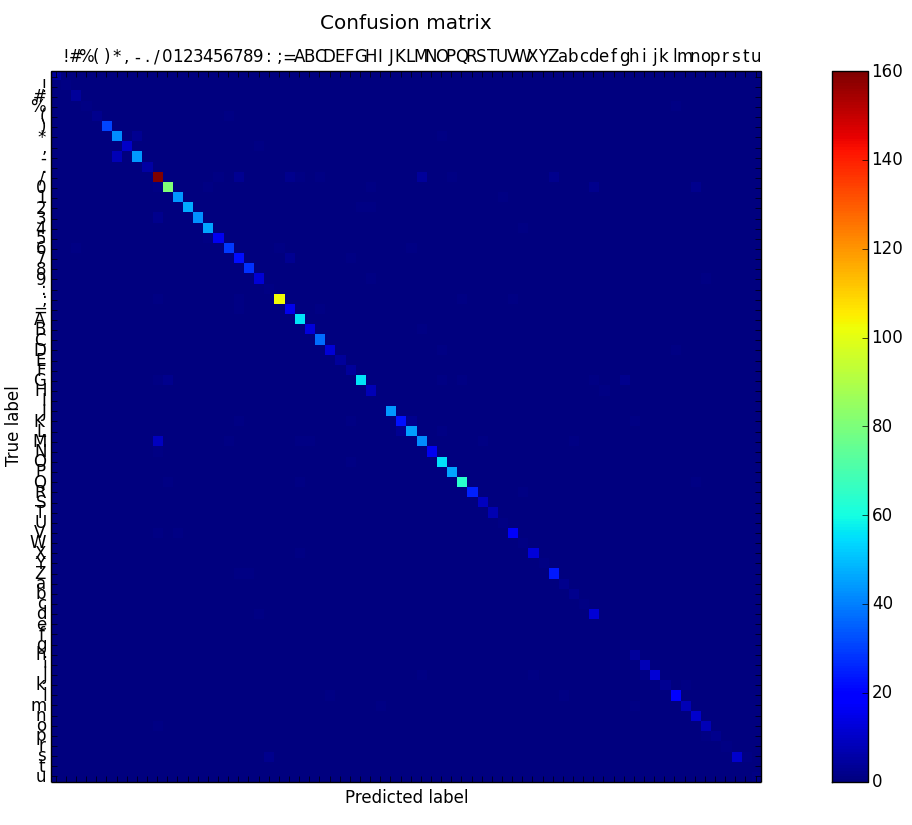
\includegraphics[width=0.8\linewidth]{img/rec_cm.png}
\caption{\label{fig:conf_matrix}
Confusion matrix for the best model for the character recognition problem}
\end{center}
\end{figure}

Table \ref{table:seg_values} contains the average, maximum and minimum values obtained for the F1 measure\cite{fawcett2006introduction} of the character segmentation problem. The F1 measure is used instead of the accuracy because the two classes are imbalanced: there are 11475 data points which indicate a segmentation point, while there are 19402 points which are not segmentation points, almost twice as many. 

\begin{table}[h]
\caption{The F1 score for the character segmentation experiment}
\label{table:seg_values}
\begin{tabular}{llllll}
\toprule
Nr. trees & Nr. features & Min     & Max     & Mean    & Std. dev. \\ 
\midrule
150 & 20 & 0.87318 & 0.88326 & 0.87735 & 0.00363 \\ 
200 & 20 & 0.86975 & 0.88312 & 0.87657 & 0.00490 \\ 
250 & 20 & 0.87258 & 0.88776 & 0.87773 & 0.00531 \\ 
150 & 8 & 0.86894 & 0.88376 & 0.87569 & 0.00517 \\ 
200 & 8 & 0.87227 & 0.88299 & 0.87675 & 0.00413 \\ 
250 & 8 & 0.87178 & 0.88470 & 0.87717 & 0.00426 \\ 
150 & 120 & 0.87262 & 0.88631 & 0.87816 & 0.00476 \\ 
200 & 120 & 0.87122 & 0.88387 & 0.87724 & 0.00418 \\ 
250 & 120 & 0.87367 & 0.88565 & 0.87885 & 0.00391 \\ 
150 & 40 & 0.87073 & 0.88671 & 0.87822 & 0.00552 \\ 
200 & 40 & 0.86980 & 0.88519 & 0.87845 & 0.00513 \\ 
250 & 40 & 0.87358 & 0.88671 & 0.87936 & 0.00445 \\ 
\bottomrule
\end{tabular}
\end{table}

The confusion matrix for the best experiment on the character segmentation problem is presented in table \ref{table:seg_conf}.

\begin{table}[h]
\caption{The confusion matrix for the character segmentation experiment}
\label{table:seg_conf}
\begin{tabular}{lll}
\hline
 & No split & Split \\ \hline
Predicted no split & 4556 & 363 \\ 
Predicted split & 255 & 2546 \\  \hline
\end{tabular}
\end{table}

In table \ref{table:line_identify}
\begin{table}[h]
\caption{The confusion matrix for the line identification problem}
\label{table:line_identify}
\begin{tabular}{lrrrrrrrrr}
\toprule
{} &  Address &  CUI &  Data &  Name &  Price &  Shop &  Total &  TVA &  Misc. \\
\midrule
Address &       62 &    0 &     0 &     3 &      0 &     0 &      0 &    0 &        0 \\
CUI     &        0 &   50 &     0 &     2 &      0 &     0 &      0 &    0 &        5 \\
Data    &        0 &    0 &    53 &     0 &      0 &     0 &      0 &    0 &        2 \\
Name    &        0 &    0 &     0 &   169 &      2 &     0 &      0 &    0 &       43 \\
Price   &        0 &    2 &     0 &     0 &    173 &     0 &      0 &    0 &        6 \\
Shop    &        0 &    0 &     0 &     0 &      0 &    55 &      0 &    0 &        0 \\
Total   &        0 &    0 &     0 &     0 &      0 &     0 &     79 &    0 &        0 \\
TVA     &        0 &    0 &     0 &     1 &      0 &     0 &      0 &   68 &        0 \\
Misc.   &        5 &    5 &     3 &     8 &      8 &     3 &      2 &    0 &      580 \\
\bottomrule
\end{tabular}
\end{table}

\section{Development}

% trebuie referinte la Python, scikit-learn, Django si alte librarii?
ReceiptBudget is a web application written in Python, using the Django framework. The dashboard was developed using the Google Maps API v3, the d3.js and dc.js Javascript visualization frameworks and the crossfilter Javascript data filtering library. 

For the processing of the image the OpenCV libray is used, with its Python bindings. The scikit-learn library \cite{pedregosa2011scikit} is used for the random forest and SVM implementations, while the neural networks are used from the pylearn2 library \cite{goodfellow2013pylearn2}. 
\subsection{Requirements Analysis}
The application needs to support multiple users. New users can create an account by registering. After that they can import a CSV file that was exported from other finance management software. 

An authenticated user can then start inserting his expenses. He has three ways to do this. The first one is to take a picture of the receipt using a webcam. The second is to upload a photo containg a receipt from his harddrive. The last option is to enter the details of the receipt manually. 

In the dashboard, the user has three views where he can visualize his expenses. He can see a heat map of all his expenses. Another view is a dynamic heat map that shows the progression of his expenses day by day. The last view is the one which contains the interactive charts and graphs. Here the user can see detailed breakdowns of his expenses by day of week, shop, months and date range, hopefully noticing any negative spending patterns that can be cut down. 

If a users expenses for the past week are over the average weekly expenses, they will receive a visual warning, reminding them to be careful with what they spend their money on. This warning comes as a bright colored bar at the top of the screen, with the intensity of the color depending on how much the user stepped over the normal expense range. 
\subsection{Design}
\subsection{Implementation}
\subsection{User Manual}
\label{sec:manual}
\section{Discussion}